\documentclass[11pt,preprint, authoryear]{elsarticle}

\usepackage{lmodern}
%%%% My spacing
\usepackage{setspace}
\setstretch{1.2}
\DeclareMathSizes{12}{14}{10}{10}

% Wrap around which gives all figures included the [H] command, or places it "here". This can be tedious to code in Rmarkdown.
\usepackage{float}
\let\origfigure\figure
\let\endorigfigure\endfigure
\renewenvironment{figure}[1][2] {
    \expandafter\origfigure\expandafter[H]
} {
    \endorigfigure
}

\let\origtable\table
\let\endorigtable\endtable
\renewenvironment{table}[1][2] {
    \expandafter\origtable\expandafter[H]
} {
    \endorigtable
}


\usepackage{ifxetex,ifluatex}
\usepackage{fixltx2e} % provides \textsubscript
\ifnum 0\ifxetex 1\fi\ifluatex 1\fi=0 % if pdftex
  \usepackage[T1]{fontenc}
  \usepackage[utf8]{inputenc}
\else % if luatex or xelatex
  \ifxetex
    \usepackage{mathspec}
    \usepackage{xltxtra,xunicode}
  \else
    \usepackage{fontspec}
  \fi
  \defaultfontfeatures{Mapping=tex-text,Scale=MatchLowercase}
  \newcommand{\euro}{€}
\fi

\usepackage{amssymb, amsmath, amsthm, amsfonts}

\def\bibsection{\section*{References}} %%% Make "References" appear before bibliography


\usepackage[round]{natbib}

\usepackage{longtable}
\usepackage[margin=2.3cm,bottom=2cm,top=2.5cm, includefoot]{geometry}
\usepackage{fancyhdr}
\usepackage[bottom, hang, flushmargin]{footmisc}
\usepackage{graphicx}
\numberwithin{equation}{section}
\numberwithin{figure}{section}
\numberwithin{table}{section}
\setlength{\parindent}{0cm}
\setlength{\parskip}{1.3ex plus 0.5ex minus 0.3ex}
\usepackage{textcomp}
\renewcommand{\headrulewidth}{0.2pt}
\renewcommand{\footrulewidth}{0.3pt}

\usepackage{array}
\newcolumntype{x}[1]{>{\centering\arraybackslash\hspace{0pt}}p{#1}}

%%%%  Remove the "preprint submitted to" part. Don't worry about this either, it just looks better without it:
\makeatletter
\def\ps@pprintTitle{%
  \let\@oddhead\@empty
  \let\@evenhead\@empty
  \let\@oddfoot\@empty
  \let\@evenfoot\@oddfoot
}
\makeatother

 \def\tightlist{} % This allows for subbullets!

\usepackage{hyperref}
\hypersetup{breaklinks=true,
            bookmarks=true,
            colorlinks=true,
            citecolor=blue,
            urlcolor=blue,
            linkcolor=blue,
            pdfborder={0 0 0}}


% The following packages allow huxtable to work:
\usepackage{siunitx}
\usepackage{multirow}
\usepackage{hhline}
\usepackage{calc}
\usepackage{tabularx}
\usepackage{booktabs}
\usepackage{caption}


\newenvironment{columns}[1][]{}{}

\newenvironment{column}[1]{\begin{minipage}{#1}\ignorespaces}{%
\end{minipage}
\ifhmode\unskip\fi
\aftergroup\useignorespacesandallpars}

\def\useignorespacesandallpars#1\ignorespaces\fi{%
#1\fi\ignorespacesandallpars}

\makeatletter
\def\ignorespacesandallpars{%
  \@ifnextchar\par
    {\expandafter\ignorespacesandallpars\@gobble}%
    {}%
}
\makeatother

\newlength{\cslhangindent}
\setlength{\cslhangindent}{1.5em}
\newenvironment{CSLReferences}%
  {\setlength{\parindent}{0pt}%
  \everypar{\setlength{\hangindent}{\cslhangindent}}\ignorespaces}%
  {\par}


\urlstyle{same}  % don't use monospace font for urls
\setlength{\parindent}{0pt}
\setlength{\parskip}{6pt plus 2pt minus 1pt}
\setlength{\emergencystretch}{3em}  % prevent overfull lines
\setcounter{secnumdepth}{5}

%%% Use protect on footnotes to avoid problems with footnotes in titles
\let\rmarkdownfootnote\footnote%
\def\footnote{\protect\rmarkdownfootnote}
\IfFileExists{upquote.sty}{\usepackage{upquote}}{}

%%% Include extra packages specified by user
\usepackage{amsmath}

%%% Hard setting column skips for reports - this ensures greater consistency and control over the length settings in the document.
%% page layout
%% paragraphs
\setlength{\baselineskip}{12pt plus 0pt minus 0pt}
\setlength{\parskip}{12pt plus 0pt minus 0pt}
\setlength{\parindent}{0pt plus 0pt minus 0pt}
%% floats
\setlength{\floatsep}{12pt plus 0 pt minus 0pt}
\setlength{\textfloatsep}{20pt plus 0pt minus 0pt}
\setlength{\intextsep}{14pt plus 0pt minus 0pt}
\setlength{\dbltextfloatsep}{20pt plus 0pt minus 0pt}
\setlength{\dblfloatsep}{14pt plus 0pt minus 0pt}
%% maths
\setlength{\abovedisplayskip}{12pt plus 0pt minus 0pt}
\setlength{\belowdisplayskip}{12pt plus 0pt minus 0pt}
%% lists
\setlength{\topsep}{10pt plus 0pt minus 0pt}
\setlength{\partopsep}{3pt plus 0pt minus 0pt}
\setlength{\itemsep}{5pt plus 0pt minus 0pt}
\setlength{\labelsep}{8mm plus 0mm minus 0mm}
\setlength{\parsep}{\the\parskip}
\setlength{\listparindent}{\the\parindent}
%% verbatim
\setlength{\fboxsep}{5pt plus 0pt minus 0pt}



\begin{document}



\begin{frontmatter}  %

\title{The Link Between Market Correlation Structure and the Performance of
Risk-Based Portfolios}

% Set to FALSE if wanting to remove title (for submission)




\author[Add1]{Nathan Potgieter\footnote{\textbf{Contributions:} \newline \emph{The
  author would like to thank Nico Katzke for helping me puzzle and prod
  my to to the eventual completion of this research project.}}}
\ead{19959672@sun.ac.za}





\address[Add1]{Stellenbosch University, Stellenbosch, South Africa}


\begin{abstract}
\small{
This work uses Monte Carlo methods to design and simulate financial
market returns for five distinctive markets types, with each market type
possesing a unique correlation structure. The equal weight, minimum
variance, inverse variance, equal risk contribution and maximum
diversification risk-based portfolios are evaluated in each of the
simulated markets. The relative performance of each of the portfolios
are compaired within market types and the relationship between each
portfolio's return characteristics and the market covariance structure
is evaluated. \textbf{FINDINGS}
}
\end{abstract}

\vspace{1cm}

\begin{keyword}
\footnotesize{
Monte Carlo \sep Risk-based Portfolios \sep Portfolio Selection
\sep Copula \\ \vspace{0.3cm}
\textit{JEL classification} L250 \sep L100
}
\end{keyword}
\vspace{0.5cm}
\end{frontmatter}



%________________________
% Header and Footers
%%%%%%%%%%%%%%%%%%%%%%%%%%%%%%%%%
\pagestyle{fancy}
\chead{}
\rhead{}
\lfoot{}
\rfoot{\footnotesize Page \thepage}
\lhead{}
%\rfoot{\footnotesize Page \thepage } % "e.g. Page 2"
\cfoot{}

%\setlength\headheight{30pt}
%%%%%%%%%%%%%%%%%%%%%%%%%%%%%%%%%
%________________________

\headsep 35pt % So that header does not go over title




\hypertarget{introduction}{%
\section{\texorpdfstring{Introduction
\label{Introduction}}{Introduction }}\label{introduction}}

Since Harry Markovitz's (1952) seminal work on mean-variance portfolios
scholars from around the globe have been aspiring to develop a robust
algorithm capable of situating a portfolio on the efficient frontier
\emph{ex ante}. There are now a wide array of available portfolio
algorithms raging from simple heuristic based approaches to advanced
mathematical algorithms based on quadratic optimization, random matrix
theory and machine learning methods; with many more are still to come.

Unfortunately, portfolio optimisers of Markowitz
(\protect\hyperlink{ref-markowitz}{1952}) mean-variance type suffer from
seveer sensitivity issues, where slight changes in their expected return
input cause large changes in optimal portfolio weights. This is
exacerbated by the fact that expected returns are notoriously difficult,
if not impossible, to accurately forecast (De Prado,
\protect\hyperlink{ref-lopez}{2016}). Due to this issue, this work
focuses solely on the so-called risk-based portfolio, defined by De
Carvalho \emph{et al.}
(\protect\hyperlink{ref-leote}{2012}\protect\hyperlink{ref-leote}{a}) as
``systemic quantitative approaches to portfolio allocation'' that solely
rely on views of risk when allocating capital. These strategies do not
require expected return forecasts and are therefore said to be more
robust to estimation error. Despite their sole focus on risk mitigation
empirical back tests have shown that they often perform surprising well,
form a total return standpoint (Choueifaty \emph{et al.},
\protect\hyperlink{ref-choueifaty2013}{2013}).

Rather than using the standard empirical approach to evaluating said
strategies this work opts to use Monte Carlo simulation methods. This
also allows for an investigation of the link between the markets
covariance structure and portfolio performance. Monte Carlo methods
prove to be invaluable in answering this question as they allow for the
creation of \emph{ad hoc} markets with predetermined risk return
characteristics, and hence leave no uncertainty regarding the
composition of the market. This creates an environment ideal for
experimentation as the researcher has complete control over the market
and can therefore adjust the independent variable, in this case the
markets correlation structure, and observe the response in the dependent
variable, which in this study is the portfolio return series. Monte
Carlo methods are also beneficial here because they enable the effective
reduction of noise in portfolio performance measures.

The risk-based portfolios evaluated in this work include the naive equal
weight (EW), minimum variance (MV), inverse variance (IV), equal risk
contribution (ERC) and the maximum diversification (MD) portfolios.
Section \ref{aims} lays out this works aims and objects. Section
\ref{lit} provides a review of the relevant literature; this includes
some general issues plaguing the field of portfolio optimization, the
rational and theoretical underpinnings behind the five risk-based
portfolios, their relative performance in empirical back tests and
finally the importance of using Monte Carlo methods in finance. Section
\ref{methadology} discusses this works methodology, Section
\ref{reasults} provides and discusses the results, and finally Section
\ref{conclusion} concludes.

\hypertarget{aims-and-objectives}{%
\section{\texorpdfstring{Aims and Objectives
\label{aims}}{Aims and Objectives }}\label{aims-and-objectives}}

This work aims to use Monte Carlo Methods to uncover the relationship
between a market's correlation structure and the risk return properties
of various risk-based portfolio algorithms. This is achieved through the
following objectives:

\begin{enumerate}
\def\labelenumi{\arabic{enumi}.}
\item
  Design and create four distinctive \emph{ad hoc} correlation matrices
  and estimate one empirical correlation matrix, each describing a
  market of 50 assets with a unique correlation structure. These market
  range from those possessing no clusters to those exhibiting
  hierarchical clustering. All other risk characteristics remain equal
  between market types.
\item
  Use these five correlation matrices as the key input in their own
  Monte Carlo simulation. Where each correlation matrix corresponds to a
  unique market type. The markets will each be built with a student t
  multivariate distribution with 4.5 degrees of freedom. The individual
  asset's univariate distributions will each be normally distributed
  with means and standard deviations calibrated with S\&P500 data. Each
  of the five market types will be simulated 10 000 times across 500
  periods, or approximately two years of trading daily return data.
\item
  Calculate the returns obtained from various risk based portfolio's in
  each of the simulated markets. Use the first \textbf{250} periods to
  estimate an out of sample covariance matrix and calculate portfolio
  weights. Conduct periodic rebalancing every 50 periods, each time
  looking back \emph{250} periods, recalculating the covariance matrix
  and the new portfolio weights. Repeat this process until all
  \emph{500} simulated periods have been considered.
\item
  Calculate the average Sharp ratio, standard deviation, downside
  deviation, value at risk (VaR), effective number of constitutes (ENC)
  and effective number of bets (ENB) for each portfolio across the 10
  000 markets for each market type.
\item
  Compare the relative performance of each portfolio within each of the
  market types and evaluate how the relative performance of each
  portfolio is effected by the change in market correlation structure.
\end{enumerate}

\hypertarget{litrature-review}{%
\section{\texorpdfstring{Litrature Review
\label{lit}}{Litrature Review }}\label{litrature-review}}

\hypertarget{a-review-of-portfolio-optimisation-algorithms}{%
\subsection{A Review of Portfolio Optimisation
Algorithms}\label{a-review-of-portfolio-optimisation-algorithms}}

\hypertarget{introduction-1}{%
\subsubsection{Introduction}\label{introduction-1}}

This literature review will cover some common issues found in the
literature surrounding portfolio optimization, the five risk-based
portfolios evaluated in this work, their respective performance in both
empirical back tests and Monte Carlo studies and finally the importance
of using Monte Carlo methods within the field of finance.

\hypertarget{common-issues-portfolio-optimizers}{%
\subsubsection{Common Issues Portfolio
Optimizers}\label{common-issues-portfolio-optimizers}}

When operating in sample, Portfolio optimization tends to be a perfect
science, but out of sample it becomes more of an art form where it is
often preferable to use heuristic over hard rules. This section
highlights some general issues, highlighted within the portfolio
optimization literature, that tend to worsen their performance out of
sample.

Firstly, mean-variance optimisers, like those introduced by Markowitz
(\protect\hyperlink{ref-markowitz}{1952}), rely heavily on the accuracy
of their expected return forecasts. Small changes in their expected
return input can lead to large changes in portfolio weights (De Prado,
\protect\hyperlink{ref-lopez}{2016}). Since in practice expected returns
are extremely difficult to accurately estimate, this issue serves as a
major hindrance to their wide spread use. Due to this the so-called risk
based portfolios that intentionally avoid using expected return
forecasts have garnered a lot of attention (Maillard,
\protect\hyperlink{ref-maillard2010}{2010}).

However, these risk based portfolios are not void of issues. The
quadratic programming methods used in many portfolio optimisers,
including Markovitz's (1952) mean variance and some risk-based
portfolios, require the inversion of some positive-definite covariance
matrix. This requirement for positive definiteness can cause issues as
covariance matrices estimated on empirical data are sometimes not
positive definite, in which case their inverse does not exist and these
portfolios don't have solutions (De Prado,
\protect\hyperlink{ref-lopez}{2016}). A common method to get around this
issue is to simply compute the nearest positive definite matrix and use
that instead (Bates \& Maechler, \protect\hyperlink{ref-Matrix}{2019};
Higham, \protect\hyperlink{ref-higham2002}{2002}).

The covariance estimation step is particularly susceptible to
measurement error if the underlying covariance matrix suffers from a
high condition number (Zhou \emph{et al.},
\protect\hyperlink{ref-zhou2019}{2019}). A condition number is defined
as the absolute value of the ratio between a covariance matrix's largest
and smallest eigenvalues (Bailey \& Lopez De Prado,
\protect\hyperlink{ref-lopez2012}{2012}; De Prado,
\protect\hyperlink{ref-lopez}{2016}). The condition number is smallest
in diagonal matrices (they have a condition number of 1) and increases
as more correlated variables are added. When working with high condition
number matrices a small change in a single entry's estimated covariance
can greatly alter its inverse, which in turn can effect the portfolio
weights (De Prado, \protect\hyperlink{ref-lopez}{2016}). This is related
to Markowitz's curse which De Prado
(\protect\hyperlink{ref-lopez}{2016}) summerised by stating that ``the
more correlated investments are, the greater is the need for a
diversified portfolio---and yet the greater are that portfolio's
estimation errors''.

For a sample with a given number of periods, larger dimension covariance
matrices are prone to more noise in estimation. This is essentially due
to a reduction in degrees of freedom as a sample of at least
\(1/2N(N+1)\) independent and identically distributed (iid) observations
are required to estimate an \(N\times N\) covariance matrix (De Prado,
\protect\hyperlink{ref-lopez}{2016}: 60){]}. Furthermore, financial
market covariance structures tend to vary over time and have been know
to change rapidly during so-called regime changes (De Prado,
\protect\hyperlink{ref-lopez}{2016}). This exacerbates the issue of
requiring a large number of observations when estimating the covariance
matrix, since passed data may not be a good refection of the future and
looking further into the passed increases this likelihood.

\hypertarget{risk-based-portfolios}{%
\subsubsection{Risk Based Portfolio's}\label{risk-based-portfolios}}

This section reviews the intuition and technical underpinnings within
the literature surrounding risk-based portfolios. Those discussed here
include the equal weight (EW), minimum variance (MV), inverse volatility
(IV), equal risk contribution (ERC) and the maximum diversification (MD)
portfolios. The EW is a simple heuristic approach, the minimum variance
is more akin to a Markovitz (1952) mean variance portfolio, while the
inverse-variance (IV), equal risk contrition (ERC) and maximum
diversification (MD) are quite similar in that they all assume that
adequate diversification can be obtained by allocating equal risk to
each investible security.

\hypertarget{naive-equal-weight-ew}{%
\paragraph{Naive Equal Weight (EW)}\label{naive-equal-weight-ew}}

Perhaps the oldest and most simple portfolio diversification heuristic
involves holding a weight of \(1/N\) of the \(N\) total available assets
(DeMiguel \emph{et al.}, \protect\hyperlink{ref-demiguel2009}{2009}). In
other words this strategy can be described as putting an equal number of
eggs into each available basket. It doesn't require any historical data
when allocating capital and doesn't involve any form of optimization
(DeMiguel \emph{et al.}, \protect\hyperlink{ref-demiguel2009}{2009}).
This portfolio is commonly called the equal weight or 1/N portfolio,
however its failure to recognize the importance of both asset variance
and the covariance between assets has resulted in it also being referred
to as the naive portfolio. Meanwhile its simplicity means that it has
been widely used as a benchmark. Equal weighting is optimal from a mean
variance standpoint when there is no correlation between securities and
each possesses the same variance. In which case, the EW is theoretically
equivalent to the MV portfolio. The EW's robustness to estimation errors
and surprisingly good historical performance has lead to it being
incorporated into hybrid portfolio strategies (Tu \& Zhou,
\protect\hyperlink{ref-tu2011}{2011}). These strategies form a balance
between the rules based approach of the EW and the optimization
approaches from more sophisticated portfolios and have been shown to
outperform both its EW and more sophisticated constituents.

\hypertarget{minimum-variance-mv}{%
\paragraph{Minimum Variance (MV)}\label{minimum-variance-mv}}

Portfolio optimisers designed to exhibit the minimum variance have in
recent years garnered a lot of attention. This can in large part be
attributed to their tendency to achieve surprisingly high returns and
low variance in historical back tests (Clarke \emph{et al.},
\protect\hyperlink{ref-clarke2011}{2011}). Their excelent performance
has been attributed to the empirical phenomena that low volatility
stocks tend to earn returns in excess of the market, and high beta
stocks tend not to be rewarded by higher returns (Clarke \emph{et al.},
\protect\hyperlink{ref-clarke2011}{2011}; Fama \& French,
\protect\hyperlink{ref-fama1992}{1992}). Interesting this later finding
is contrary to traditional financial economic theory which predicts an
asset's expected return to be proportional to its market beta
(i.e.~undiversifiable risk) (Perold,
\protect\hyperlink{ref-perold2004}{2004}).

The minimum variance portfolio selects security weights such that the
resulting portfolio corresponds to that with the lowest possible in
sample volatility. Therefore, it has the lowest expected volatility and
is, in theory, the safest/least risky portfolio (De Carvalho \emph{et
al.},
\protect\hyperlink{ref-rawl2012}{2012}\protect\hyperlink{ref-rawl2012}{b}).
Its primary input is a variance covariance matrix, which it uses to
minimize aggregate portfolio volatility. This is accomplished by
over-weighting low volatility and low correlation securities (De
Carvalho \emph{et al.},
\protect\hyperlink{ref-rawl2012}{2012}\protect\hyperlink{ref-rawl2012}{b}).
Interestingly, it is the only portfolio of the efficient frontier that
does not depend on expected return forecasts (De Prado,
\protect\hyperlink{ref-lopez}{2016}).

Let \(\sum\) indicate the markets variance covariance matrix and
\(w=\{w_i,..., w_N \}\) be a vector of length N containing individual
security weights. The vector containing the MV portfolio's weights can
now be described as (De Carvalho \emph{et al.},
\protect\hyperlink{ref-rawl2012}{2012}\protect\hyperlink{ref-rawl2012}{b}):

\begin{center}
$w^*=arg\min(w'\sum w)\ \ \ s.t.\ \sum^N_iw_i=1$ 
\end{center}

In some studies the minimum variance (MV) portfolio has been found by to
earn cumulative returns equal to or slightly greater than market
capitalization weighted portfolio's whilst maintaining a consistently
lower variance and achieving a noticeable improvement in downside risk
mitigation (Clarke \emph{et al.},
\protect\hyperlink{ref-clarke2011}{2011}). The MV portfolio can
therefore work well out of sample, but if left unrestricted is known to
build highly concentrated portfolio's (De Prado,
\protect\hyperlink{ref-lopez}{2016}). Its sole objective to minimize
portfolio volatility is likely the the primary reason for this. When
near the trough of its objective function it to achieves minor
reductions in \emph{ex ante} volatility by greatly favoring a small
number of low volatility/correlation securities (De Prado,
\protect\hyperlink{ref-lopez}{2016}: 68){]}. This tendency to produce
highly concentrated portfolio's can be costly out of sample as the
portfolio does not sufficiently diversify its idiosyncratic risk. It
puts too many eggs in too few baskets. In practice This issue can be
countered by applying cleaver maximum and minimum portfolio weight
constraints.

\hypertarget{inverse-varience-iv-weighting}{%
\paragraph{Inverse-Varience (IV)
Weighting}\label{inverse-varience-iv-weighting}}

The IV portfolio, referred to as the equal-risk budget (ERB) portfolio
in De Carvalho \emph{et al.}
(\protect\hyperlink{ref-leote}{2012}\protect\hyperlink{ref-leote}{a}),
aims to allocate an equal risk budget to each investible security (De
Carvalho \emph{et al.},
\protect\hyperlink{ref-leote}{2012}\protect\hyperlink{ref-leote}{a}).
Where the risk budget is defined as the the product of a security's
weight and volatility. If \(\sigma_i\) is defigned as security i's
volatility, then risk the portfolio risk budget can be equally
distributed across N securities by setting security weights as:

\begin{center} 
$w_{iv}=(\frac{1/\sigma_1}{\sum^N_{j=1} 1/\sigma}, ...,\frac{1/\sigma_N}{\sum^N_{j=1} 1/\sigma} )$ 
\end{center}

This indicates that each securities weight is directly proportional to
the inverse of its variance, thereby demonstrating why this is called
the IV portfolio. The IV portfolio allocates capital based solely on
security variance and is therefore oblivious to the covariance between
its constitutes. De Carvalho \emph{et al.}
(\protect\hyperlink{ref-leote}{2012}\protect\hyperlink{ref-leote}{a})
found that, if all securities posses the same sharp ratio and their
correlation coefficients are all equal, then the IV portfolio is
efficient from a mean variance stand point and obtains the highest
possible sharp ratio.

\hypertarget{equal-risk-contribution-erc}{%
\paragraph{Equal Risk Contribution
(ERC)}\label{equal-risk-contribution-erc}}

The principle behind the ERC portfolio is similar to that of the IV,
however when balancing risk contributions the ERC does account for the
covariance between securities (De Carvalho \emph{et al.},
\protect\hyperlink{ref-leote}{2012}\protect\hyperlink{ref-leote}{a}).
The ERC allocates capital such that each security contributes equally to
overall portfolio risk, which in theory should maximize risk
diversification (Maillard, \protect\hyperlink{ref-maillard2010}{2010}).
In practice the ERC acts similar to a weight constrained MV portfolio,
with constraints preventing high levels of portfolio concentration.
Following Maillard (\protect\hyperlink{ref-maillard2010}{2010}), the
weights of an ERC portfolio \(x=(x_1,x_2,...,x_n)\) consisting of n
assets can be calculated as follows:

let \(\sigma_i^2\) resemble asset i's variance, \(\sigma_{ij}\) the
covariance between asset i and j and \(\sum\) be the markets variance
covariance matrix. Portfolio risk can now be written as
\(sigma(x)=\sqrt{x^T\sum x}=\sum_i\sum_{j\neq i}x_ix_j\sigma_{ij}\) and
the marginal risk contribution, \(\partial_{x_i}\sigma(x)\), can then be
defined as:

\begin{center}
$\partial_{x_i}\sigma(x)=\frac{\partial\sigma(x)}{\partial x_i}=\frac{x_i\sigma_i^2+\sum_{j\neq i}x_j\sigma_{ij}}{\sigma(x)}$ 
\end{center}

Therefore, \(\partial_{x_i}\sigma(x)\) refers to the change in portfolio
volatility resulting from a small change in asset i's weight (Maillard,
\protect\hyperlink{ref-maillard2010}{2010}). ERC uses this definition to
guide central objective to equate the risk contribution across each of
the n asset. There is no closed form solution describing the weights of
the ERC portfolio, however, if we define \((\sum x)_i\) as the
\(i^{th}\) row resulting from the product of \(\sum\) with x and note
that \(\partial_{x_i}\sigma(x)=(\sum x)_i\), then the optimal weight for
the long only ERC can be described as those that satisfy the following
statement (see Maillard (\protect\hyperlink{ref-maillard2010}{2010}),
p.~4-7 for more detail):

\begin{center}
$x^*=\{x \ \epsilon[0,1]^n:\sum x_i=1, x_i \times (\sum x)_i=x_j \times (\sum x)_j \ \forall  \ i,j \}$ 
\end{center}

Maillard (\protect\hyperlink{ref-maillard2010}{2010}) proved
mathematically that the ERC portfolio's \emph{ex ante} volatility is
always some where between those of the EW and MV portfolio's. De
Carvalho \emph{et al.}
(\protect\hyperlink{ref-leote}{2012}\protect\hyperlink{ref-leote}{a})
found that, if all securities posses the same sharp ratio , then the ERC
and ERB have identical portfolio weights. If in addition the correlation
coefficients between all securities are equal, then the ERC and ERB
merge into the EW portfolio, with each being mean variance efficient
with the maximum attainable sharp ratio (De Carvalho \emph{et al.},
\protect\hyperlink{ref-leote}{2012}\protect\hyperlink{ref-leote}{a}).

\hypertarget{maximum-diversification-md}{%
\paragraph{Maximum Diversification
(MD)}\label{maximum-diversification-md}}

Choueifaty \& Coignard (\protect\hyperlink{ref-choueifaty2008}{2008})
originally designed the MD portfolio to maximize some diversification
ratio (D), which he defined as the sum of each securities risk bucket
(\(w'.V\)) divided by portfolio volatility (De Carvalho \emph{et al.},
\protect\hyperlink{ref-leote}{2012}\protect\hyperlink{ref-leote}{a}). If
we define V as a vector of asset volatilities and \(\sum\) as the
covariance matrix and \(w^*\) as the vector of MD portfolio weight. Then
the \(w*\) can be expresses as:

\begin{center} 
$w^* =arg\ max(DR)\ \ \ \ with \ \ \ \  DR= \frac{w'.V}{\sqrt{w'Vw}}$ 
\end{center}

De Carvalho \emph{et al.}
(\protect\hyperlink{ref-leote}{2012}\protect\hyperlink{ref-leote}{a})
found that in practice the MV achieves a diversification ratio similar
to that of the MD and that the difference between the two arise from the
difference between the two arise from the MV's larger exposure to low
residual volatility securities. Much like the IV and ERC portfolios, the
MD portfolio attempts to diversify its portfolio by allocating equal
risk to each security (Choueifaty \& Coignard,
\protect\hyperlink{ref-choueifaty2008}{2008}). The MD portfolio
accomplishes this by over-weighting low volatility and low correlation
securities (De Carvalho \emph{et al.},
\protect\hyperlink{ref-leote}{2012}\protect\hyperlink{ref-leote}{a}).
For further detail regarding the theoretical results and properties of
the MD portfolio see Choueifaty \& Coignard
(\protect\hyperlink{ref-choueifaty2008}{2008}: 33--35).

\hypertarget{empirical-backtests-and-monte-carlo-findings}{%
\subsection{Empirical Backtests and Monte Carlo
Findings}\label{empirical-backtests-and-monte-carlo-findings}}

Choueifaty \emph{et al.} (\protect\hyperlink{ref-choueifaty2013}{2013})
used empirical back testing to compare the relative performance of
numerous portfolio optimisers. They used historical data from the MSCI
world index and considered the largest 50\% of assets at each
semi-annual rebalance date between 1999 and 2010. To reduce the noise in
estimation, at each rebalance date covariance matrices were estimated
using the previous years worth of data (Choueifaty \emph{et al.},
\protect\hyperlink{ref-choueifaty2013}{2013}). These were then used as
the primary inputs in estimating the long-only portfolio weights. The MV
portfolio achieved an annual return of 6.7\% and outperformed the ERC
and EW portfolios who returned 6.3\% and 5.8\% respectively. The MV
portfolio possessed the lowest daily volatility (10\%) followed by the
ERC and then the EW portfolio's (with 12.9\% and 16.4\% respectively).
Accordingly the MV portfolio had the highest sharp ratio (0.36) followed
by the ERC and EW portfolios (0.24 and 0.16 respectively).

Despite the EW portfolio simplistic nature empirical studies, like those
by DeMiguel \emph{et al.} (\protect\hyperlink{ref-demiguel2009}{2009}),
who compared the EW to the mean-variance, MV and Bayes-Stein portfolios,
tend to find a statistically insignificant difference in Sharp ratio
between the naive portfolio and those of the more advanced portfolio
optimisers.In addition the EW also performed surprisingly well from a
total return perspective. In fact many studies have found that the EW
portfolio outperforms the mean variance and other more sophisticated
portfolios based in financial theory (Tu \& Zhou,
\protect\hyperlink{ref-tu2011}{2011}).

Due to the aforementioned issues surrounding covariance matrix
estimation error, Ardia \emph{et al.}
(\protect\hyperlink{ref-ardia2017}{2017}) set out to evaluate the impact
of covariance matrix misspecification on the properties of risk based
portfolio's. They used Monte Carlo methods to build six distinctive
investment universes, each with a unique, variance/correlation structure
and a varying number of assets. Numerous covariance matrix estimation
techniques were then estimated on the simulated data, one of which
serving as the benchmark. They then used the simulated data and the
various covariance matrices to access the impact of alternative
covariance specifications on the performance of the MV, IV, ERC and MD
portfolio's. The ERC and IV portfolios were found to be ``relatively
robust to covariance misspecification'', the MV was found to be
sensitive to misspecification in both the variance and covariance and
the MD portfolio was found to be robust to variances misspecification
but sensitive to misspecification in the covariances (Ardia \emph{et
al.}, \protect\hyperlink{ref-ardia2017}{2017}: 1).

\hypertarget{monte-carlo-methods-in-portfolio-optimisation}{%
\subsection{Monte Carlo Methods in Portfolio
Optimisation}\label{monte-carlo-methods-in-portfolio-optimisation}}

Ever since the pioneering age of computers people have shown a keen
interest in leveraging their ability to perform rapid calculations to
conduct randomized experiments (Kroese \emph{et al.},
\protect\hyperlink{ref-kroese2014}{2014}: 1). The core of Monte Carlo
simulation is in the creation of random objects and/or processes using a
computer. There are a number of reasons for doing this, but the primary
one used in this work and thereby discussed in this review is of the
sampling kind (Kroese \emph{et al.},
\protect\hyperlink{ref-kroese2014}{2014}). This typically involves the
modeling of some stochastic object or process, followed by sampling from
some probability distribution and the manipulating said sample through
some deterministic process such that the result mimics the true
underlying process. The primary idea behind Monte Carlo simulation is to
repeat this simulation process many times so that interesting properties
can be uncovered through the law of large numbers and central limit
theorem.

A financial application of this can be found in Wang \emph{et al.}
(\protect\hyperlink{ref-wang2012}{2012}) who designed a Monte Calro
procedure that (1) models both the time-series and cross-section
properties of financial market returns, this involves the estimation of
a random term's probability distribution function (pdf) using extreme
value theory. And (2) sampling from the modeled process to produce an
ensemble of market returns, with each exerting the same risk properties.
The simulated data can then be used in risk management and/or the
pricing of financial securities (Kroese \emph{et al.},
\protect\hyperlink{ref-kroese2014}{2014}; Wang \emph{et al.},
\protect\hyperlink{ref-wang2012}{2012}). This unique ability to generate
a large number of counterfactuals for an asset market with a known risk
structure has made it a uniquely powerful tool in accessing the
properties of portfolio optimization algorithms (Bailey \& Lopez De
Prado, \protect\hyperlink{ref-lopez2012}{2012}).

Glasserman (\protect\hyperlink{ref-glasserman2013}{2013}) is a useful
source for understanding the methods and applications of Monte Carlo
methods in finance.

\hypertarget{methadology}{%
\section{\texorpdfstring{Methadology
\label{methadology}}{Methadology }}\label{methadology}}

This work used Monte Carlo simulation methods to investigate the link
between a markets correlation structure and the relative performance of
the EW, MV, IV, ERC and MD portfolios. To avoid possible confusion note
the following terminology:

\begin{itemize}
\tightlist
\item
  The term market refers to a set daily returns for a number of assets.
  e.g.~the daily returns for each of the JSE ALSI constitutes between 1
  January 2019 and 1 January 2020. Since this is a Monte Carlo study,
  thousands of markets are simulated, they can therefore be thought of
  as a single observation from a population of markets.
\item
  The term market type refers to a population of markets each with the
  same specified risk characteristics.
\end{itemize}

The R package MCmarket was used to simulate 10 000 markets from five
separate market types, with the correlation structure being the only
differentiating factor between between market types. (Potgieter,
\protect\hyperlink{ref-MCmarket}{2020}). Four of the correlation
structures/matrices were designed \emph{ad hoc}, while the fifth was
estimated using S\&P 500 data. These correlation matrices range from one
exhibiting no correlation (i.e.~a diagonal matrix) to one with a
hierarchical clustering structure (see \ref{corr_struc}).

The long only EW, MV, IV, ERC and MD portfolios were then back tested on
the simulated markets (Section \ref{backtest}) and portfolio analytics
were calculated and aggregated across the 10 000 markets (Section
\ref{portmet}). Finally, the portfolio metrics are compared within
market types across portfolios and within portfolios, across market
types.

\hypertarget{correlation-structures}{%
\subsection{\texorpdfstring{Correlation Structures
\label{corr_struc}}{Correlation Structures }}\label{correlation-structures}}

This section describes the composition and attributes of the four
\emph{ad hoc} correlation matrices used in this study (section
\ref{adhoc}) as well as the methodology behind the estimation of the
empirical correlation matrix (section \textbackslash ref\{emp). Each of
the five matrices top 10 eigenvalues are listed in Table \ref{eigens}.

\hypertarget{ad-hoc}{%
\subsubsection{\texorpdfstring{Ad Hoc
\label{adhoc}}{Ad Hoc }}\label{ad-hoc}}

This section describes the four \emph{ad hoc} 50 by 50 correlation
matrices used as the key inputs in their respective Monte Carlo
simulations. See Figure \ref{corr_mats} for a graphical representation
of each correlation matrix. Note that the \emph{gen\_corr} function from
the R package \emph{MCmarket} was used in the construction of the four
\emph{ad hoc} matrices (Potgieter,
\protect\hyperlink{ref-MCmarket}{2020}).

The first and most simplistic of the four matrices is a diagonal matrix
(see Diagonal Matrix in Figure \ref{corr_mats}). It describes a market
with a zero correlation coefficient between each asset. Each of its 50
eigenvalues are equal to 1 (Table \ref{eigens}), it has no risk clusters
and has plenty scope for diversification. This correlation matrix has
the lowest possible condition number of 1. The Monte Carlo data set
constructed using this matrix will be referred to as Market 1.

The second matrix (labeled No Clusters in Figure \ref{corr_mats}) has no
risk clusters but describes a market with significant correlation
between its constituents. Each asset has a correlation of 0.9 with is
closest neighbor (i.e.~Asset 1 and 2, 5 and 6 and 11 and 12 each have a
pairwise correlation coefficient of 0.9). Correlations then diminish
exponentially by the absolute distance between the two assets (i.e.~the
correlation between Asset 1 and 5 is \(0.9^{|1-5|}=0.6561\)). Its has a
large first eigenvalue of 15.93, but they quickly diminish such that its
9th largest eigenvalue is less than 1 at 0.79 (Table \ref{eigens}). This
correlation matrix has the highest condition number of 302.4. The Monte
Carlo data set constructed using this matrix will be referred to as
Market 2.

The third matrix (labeled Five Clusters in Figure \ref{corr_mats})
contains five distinctive non-overlapping risk clusters. Assets within
the same cluster have a pairwise correlation coefficient of 0.6 while
those that are not in the same cluster are uncorrelated. ItThis
correlation matrix has a condition number of 16.1. The Monte Carlo data
set constructed using this matrix will be referred to as Market 3.

The final \emph{ad hoc} correlation matrix has three layers of
overlapping risk clusters. The first layer has 10 distinctive clusters,
within which assets have a correlation coefficient of 0.7. The second
layer has four clusters where assets that are not in same first layer
cluster have a correlation coefficient of 0.5. Assets that are in the
same third layer cluster but not clustered in layers one and two have a
correlation coefficient of 0.3. Finally, those who do not share any
cluster have a correlation coefficient of 0.05. Its largest eigenvalue
is 14.36, but they diminish fairly quickly as its third largest is only
3.3 (Table \ref{eigens}). This correlation matrix has a condition number
of 47.9. The Monte Carlo data set constructed using this matrix will be
referred to as Market 4.

Table \ref{eigens} provides a list of the ten largest eigenvalues for
each of the five correlation matrices.

\begin{figure}
\centering
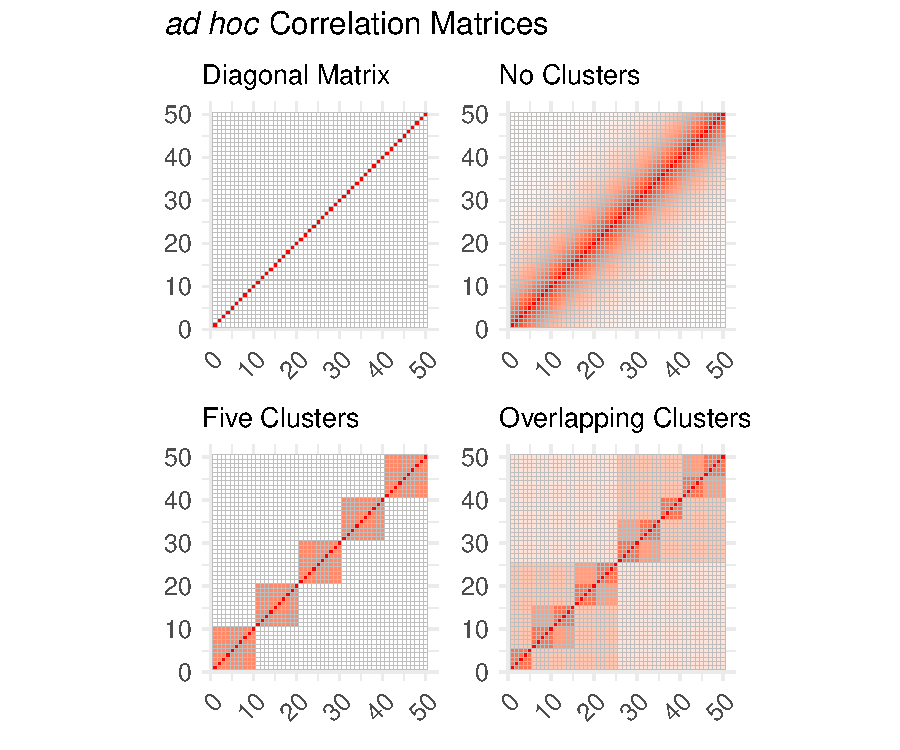
\includegraphics{Thesis_files/figure-latex/corr mats-1.pdf}
\caption{\label{corr_mats} Correlation Matricies}
\end{figure}

\hypertarget{emperical}{%
\subsubsection{\texorpdfstring{Emperical
\label{emp}}{Emperical }}\label{emperical}}

The empirical correlation matrix used in this study was estimated from
the daily returns of a random subset of 50 of the largest (by market
capitalization) 100 S\&P 500 stocks between 1 January 2016 and 1 January
2021. The market capitalizations were measured as of 12 January 2020.

The markets covariance matrix was then estimated using the
\emph{fit\_mvt} function from the R package \emph{fitHeavyTail} (Palomar
\& ZHOU, \protect\hyperlink{ref-fitHeavyTail}{2020}). This covariance
estimation method uses maximum likelihood estimation and generalized
expectation maximization to fit a multivariate t-distribution the a
matrix of asset returns (Liu \& Rubin,
\protect\hyperlink{ref-liu1995}{1995}). This procedure found that the
multivariate t distribution with 4.43 degrees of freedom and the
correlation matrix shown in Figure \ref{corr_emp} best approximated the
return series.

Note that in Figure \ref{corr_emp} assets were ordered by hierarchical
clustering so the reader could more easily visualize the risk clusters.
The correlation matrix's largest eigenvalue is 18.6 and they quickly
diminish to below zero by its 8th largest eigenvalue (Table
\ref{eigens}). This correlation matrix has a condition number of 211.1.
The Monte Carlo data set constructed using this matrix will be referred
to as Market 5.

\begin{figure}
\centering
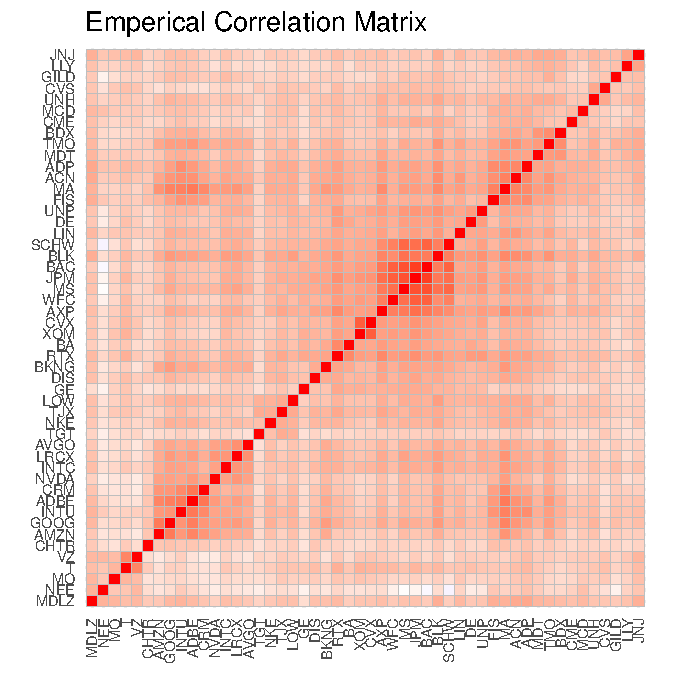
\includegraphics{Thesis_files/figure-latex/unnamed-chunk-1-1.pdf}
\caption{\label{corr_emp} Emperical Correlation Matrix}
\end{figure}

\begin{table}[!htbp] \centering 
  \caption{Eigenvalues} 
  \label{eigens} 
\begin{tabular}{@{\extracolsep{5pt}} ccccc} 
\\[-1.8ex]\hline 
\hline \\[-1.8ex] 
Diagonal & No Clusters & Five Clusters & Overlapping Clusters & Emperical \\ 
\hline \\[-1.8ex] 
1 & 15.93 & 6.4 & 14.36 & 18.6 \\ 
1 & 10.38 & 6.4 & 6.89 & 3.09 \\ 
1 & 6.28 & 6.4 & 3.3 & 2.52 \\ 
1 & 3.92 & 6.4 & 3.3 & 1.4 \\ 
1 & 2.59 & 6.4 & 2.49 & 1.28 \\ 
1 & 1.81 & 0.4 & 2.46 & 1.21 \\ 
1 & 1.32 & 0.4 & 1.3 & 1.03 \\ 
1 & 1.01 & 0.4 & 1.3 & 0.92 \\ 
1 & 0.79 & 0.4 & 1.3 & 0.88 \\ 
1 & 0.64 & 0.4 & 1.3 & 0.83 \\ 
\hline \\[-1.8ex] 
\end{tabular} 
\end{table}

\hypertarget{monte-carlo}{%
\subsection{\texorpdfstring{Monte Carlo
\label{mc}}{Monte Carlo }}\label{monte-carlo}}

This section outlines the process behind the Monte Carlo simulations
performed as part of this study.

A generalized version of the Monte Carlo procedure developed in Wang
\emph{et al.} (\protect\hyperlink{ref-wang2012}{2012}) was used to
simulate five distinctive market types. This framework was build into
the R package \emph{MCmarket} which was used to conduct this project's
Monte Carlo simulations (Potgieter,
\protect\hyperlink{ref-MCmarket}{2020}). The following briefly describes
the process:

An Elliptical t copula with 4.5 degrees of freedom is used, in
conjunction with a 50 by 50 correlation matrix (Section \ref{corrs}), to
simulate 500 random uniformly distributed draws (corresponding to 500
trading days or approximately two years worth of trading days) across
the 50 assets. The uniformly distributed observations were then
transformed into normally distributed observations, via the inverted
normal cumulative distribution function (Potgieter,
\protect\hyperlink{ref-MCmarket}{2020}; Wang \emph{et al.},
\protect\hyperlink{ref-wang2012}{2012}: 3). This process was repeated 10
000 times for each of the five correlation matrices/ market types set
out in section \ref{corr_struc}. The correlation matrix is the only
distinguishing factor between market types as all other factors remain
equal. All in all, this process created 5 data sets each containing 10
000 markets with 50 assets and 500 periods.

The expected returns and standard deviation of these simulated variables
were calibrated using a random subset of 50 of the largest 100 S\&P500
stocks (discussed in Section \ref{emp_corr}) between 1 January 2020 and
1 January 2021. Maximum likelihood estimation was used to fit the
multivariate t distribution to the return series using the method
developed by Liu \& Rubin (\protect\hyperlink{ref-liu1995}{1995}). This
produced a series of estimated means and variances which were used to
calibrate the expected returns and standard deviations of the simulated
variables (see Table \ref(msd)).

\hypertarget{back-tests}{%
\subsection{\texorpdfstring{Back Tests
\label{backtest}}{Back Tests }}\label{back-tests}}

This section describes the back testing procedure used to calculate the
returns obtained by the EW, MV, IV, ERC and MD portfolios. The process
described relates to a single market and was therefore applied to each
of the 50 000 markets simulated in this study.

To remain consistent with the literature as well as the mandate for the
majority of portfolio managers, a long-only weight constraint was
applied to all portfolio's. In addition a constraint limiting the
maximum weight applied of a single security to 10\% is also applied.
This prevents some portfolios from building unreasonably highly
concentrated holdings, while remaining flexible enough to punish those
who do so. These constraints therefore act to provide a fair playing
ground for the portfolio's to compete. The back testing procedure works
as follows:

The first 250 periods, approximately equivalent to one years worth of
daily return data, are used to fit a multivariate t distribution via
maximum likelihood and estimate a covariance matrix (Liu \& Rubin,
\protect\hyperlink{ref-liu1995}{1995}). Interestingly, the identifying
assumption used in this covariance matrix estimation method, that is
that the data comes from a multivariate t distribution, is correct by
definition since this is the distribution used to simulate the data set.
The estimated covariance matrix is then used as the sole input when
calculating the weights for each of the respective risk-based
portfolios. Each portfolio holds these weights over the next 50 periods,
when they are rebalanced by looking back 250 periods, calculating the
covariance matrix and the new portfolio returns. This process is
repeated until all periods in the data set are exhausted. Since there
are 500 periods in each market, each portfolio is weighted 5 times and
250 periods of daily returns are calculated for each portfolio.

\hypertarget{portfolio-analytics}{%
\subsection{\texorpdfstring{Portfolio Analytics
\label{portmet}}{Portfolio Analytics }}\label{portfolio-analytics}}

This section describes the portfolio performance and concentration
metrics used to evaluate and compare portfolios. The Sharp ratio is used
to evaluate the risk adjusted return, while the standard deviation (SD),
downside deviation (DD) and value at risk (VaR) are used to access
portfolio risk. Finally, the effective number of constitutes, calculated
as the inverse of the Herfindahl-Hirschman index (HHI), and the
effective number of bets, calculated following Meucci
(\protect\hyperlink{ref-meucci2010}{2010}), are used to compare
diversification between portfolios (Rhoades,
\protect\hyperlink{ref-rhoades1993}{1993}).

Since Markowitz (\protect\hyperlink{ref-markowitz}{1952}) variance of
returns has been the standard measure for risk in the financial industry
(Meucci, \protect\hyperlink{ref-meucci2010}{2010}). With SD simply being
the square-root of the variance, it too is widely used and benefits due
to its relative ease in interpretation. SD is also key in calculating
the next two portfolio performance metrics described in this study,
namely the Sharp ratio and value at risk (VaR).

The Sharp ratio is a measure of a portfolio's risk adjusted returns.
Generally speaking, the Sharp ratio is calculated by dividing the
portfolio return by some measure of portfolio risk, it is therefore
interpreted as the return per unit of risk. In this work SD is used as
the measure of risk.

The 95\% VaR is another risk metric used to evaluate portfolio risk
performance in this study. It is one of the financial industry standards
for measures for downside risk and can be interpreted as the maximum
return expected from in the worst 5\% of scenarios (Peterson \& Carl,
\protect\hyperlink{ref-PerformanceAnalytics}{2020}). That is, in the
worst 5\% of scenarios, one should expect to loose at least this amount.
The particular version of VaR used here is the Gaussian VaR, which is
calculated by assuming that returns are normally \(N(\mu,\sigma)\)
distributed, where \(\mu\) and \(\sigma\) are estimated using historical
data. The probability distribution assumptions allows one to attach a
probability values to possible future portfolio returns. This assumption
can be dangerous in practice, however in this study it correct by
definition as the return series were each simulated to be normally
distributed. It should therefore result in an accurate estimate of
downside risk.

The HHI estimates portfolio concentration by by summing the the
portfolio weights squared (Rhoades,
\protect\hyperlink{ref-rhoades1993}{1993}). A portfolio with small
weights allocated evenly across a large number of securities will have
an HHI of approximately zero, while a portfolio with all its capital
invested in a single security will have the maximum HHI of 10000. The
effective number of constitutes (ENC) can then be calculated as the
inverse of the HHI, where an equally weighted portfolio with have an ENC
equal to the number of securities and more concentrated portfolio's will
have a ENC less than the number of securities. Weight based measures of
portfolio diversification are severely limited in that they are
oblivious to covariation between portfolio components. The ENC can
therefore be misleading in financial applications where portfolio
components are known to exhibit significant dependence.

Meucci (\protect\hyperlink{ref-meucci2010}{2010}) attempted to rectify
this issue when he introduced a new method to evaluate portfolio
diversification that considers the portfolio's risk structure. He used a
principle component (PC) approach to estimate the total number of
orthogonal bets within a portfolio, which he simply referred to as
principle portfolios. With this he estimated a portfolio diversification
distribution using the percentage of total portfolio variation
attributed to each principle portfolio. The effective number of
orthogonal bets (ENB) can then be calculated as the dispersion of the
diversification distribution (Meucci,
\protect\hyperlink{ref-meucci2010}{2010}: 10).

\hypertarget{results-and-discussion}{%
\section{\texorpdfstring{Results and Discussion
\label{reasults}}{Results and Discussion }}\label{results-and-discussion}}

Note that the markets simulated using the diagonal correlation matrix
described in Section \ref{adhoc} will hence forth be referred to as
Market 1. Similarly, the markets simulated using the no cluster, five
clusters, overlapping clusters and empirical correlation matrices will
be respectively referred to as Market 2, Market 3, Market 4 and Market
5. Therefore, each of the Markets 1 - 5 contain a unique correlation
structure.

\hypertarget{comparing-portfolios-within-market-types}{%
\subsection{Comparing Portfolios Within Market
Types}\label{comparing-portfolios-within-market-types}}

\hypertarget{market-1}{%
\subsubsection{Market 1}\label{market-1}}

The portfolios compared here were estimated on the markets simulated
using the diagonal correlation matrix (Figure \ref{corr_mats}). Since
there is no correlation between assets in this market type, its
simulated markets are argubaly the least realistic. According to the
portfolio risk metrics reported in Table \ref{rm1} the EW portfolio
performed the best overall. It achieved the highest average Sharp ratio
and the lowest average SD, DD and VaR. The IV portfolio was a close
second, it has the second highest Sharp ratio, tied the lowest SD,
narrowly placing second lowest in the DD and VaR metrics. The ERC ranked
the third best overall, followed by the MD and finally the MV.

Since this market type has real no correlation structure it is
unsurprising that the two portfolios that neglect using covariance
information have performed relatively well. However, since the variance
does differ between assets it would have been reasonable to assume that
the IV portfolio would be less volatile than the EW. The fact that it is
not may be due to (1) asset return variances are not being sufficiently
different and/or (2) the IV portfolio's out of sample variance forecast
not being accurate enough to reduce the IV portfolio's out of sample
risk to below that of the EW portfolio.

The MV, ERC and MD portfolios performed poorly compared to the EW and IV
portfolios. This is likely be due to there being no real dependence in
the underlying market's correlation structure. Therefore, these
portfolios are more noisy in comparison as they use spurious covariance
information when allocating capital. The EW and IV portfolio in
comparison effectively assume that there is no correlation between
assets. In Market 1 this assumption is correct by construction.

\begin{table}[!htbp] \centering 
  \caption{Market 1 - Portfolio Risk Metrics} 
  \label{rm1} 
\begin{tabular}{@{\extracolsep{5pt}} cccccc} 
\\[-1.8ex]\hline 
\hline \\[-1.8ex] 
Metric & EW & MV & IV & ERC & MD \\ 
\hline \\[-1.8ex] 
Sharp & 0.19353 & 0.13501 & 0.18341 & 0.15876 & 0.14284 \\ 
SD & 0.00386 & 0.005 & 0.00386 & 0.00447 & 0.00494 \\ 
Downside Deviation & 0.00235 & 0.00318 & 0.00236 & 0.00279 & 0.00312 \\ 
VaR & -0.00545 & -0.00735 & -0.00548 & -0.00645 & -0.00722 \\ 
\hline \\[-1.8ex] 
\end{tabular} 
\end{table}

\textbf{Table \ref{em1} contains the average portfolio concentration
metrics. Since this market's underlying correlation matrix expresses no
dependence between assets, each assets return's are in theory
orthogonal. Therefore, the EW portfolio should produce an ENB of 50,
however, the ENB reported is 17.5. This can not simply be due to it
being a noisy measure since the ENB reported in Table \ref{em1} is an
average across the 1000 ENBs estimated for each portfolio. This miss
measurement likely due to a persistent bias that arises then rotating
the returns matrix based on noise rather than signal. Since the
underlying correlation structure implies that the returns are
orthogonal, but finite sample estimates of the correlation matrix will
inevitably contain some noise, it is likely that the ENB estimate is
finding spurious principle components which is making it an unreliable
measure of diversification.}

It is also interesting it see that the ENC and ENB are at odds.
Portfolio's rated as highly diversified by the ENC measure are are rated
as relatively undiversified by the ENB and \emph{vice verse}.
Additionally, the ENC measure coincides with the portfolio risk measures
from Table \ref{rm1}, in that those with a high ENC were less volitlie.
Meanwhile, those with the most ENB were also the most volatile. This
suggests that, when operating in a market where all correlation between
assets are estimated to be approximately zero, the ENB can be very
misleading and that the ENB is most likely a better tool for measuring
concentration.

\begin{table}[!htbp] \centering 
  \caption{Market 1 - Portfolio Concentration Metrics} 
  \label{em1} 
\begin{tabular}{@{\extracolsep{5pt}} cccccc} 
\\[-1.8ex]\hline 
\hline \\[-1.8ex] 
Metric & EW & MV & IV & ERC & MD \\ 
\hline \\[-1.8ex] 
ENC & 50 & 27.2 & 47.3 & 35.6 & 28.2 \\ 
ENB & 17.5 & 22.8 & 20.1 & 18.9 & 21 \\ 
\hline \\[-1.8ex] 
\end{tabular} 
\end{table}

\hypertarget{market-2}{%
\subsubsection{Market 2}\label{market-2}}

The portfolios compared here were estimated on the markets simulated
using the no clusters correlation matrix (Figure \ref{corr_mats}).
Unlike Market 1 the average portfolio risk metrics in Table \ref{rm2} do
not indicate a clear winner. Despite having the highest average SD the
MD portfolio achieved the highest Sharp ratio. The ERC performed best in
the SD, DD and VaR measures while obtaining the second highest Sharp
ratio. The EW and IV portfolios were similar in their performance and
the MV performed poorly.

Since this market type exhibits significant correlation between its
constituents it is unsurprising to observe the EW and IV portfolios fall
out, in favor of the more sophisticated ERC and MD portfolios.

The MV portfolio has the second lowest SD, but second highest DD and
lowest sharp ratio. This demonstrates its failure to mitigate its
downside risk exposure (measured by DD and VaR) which is arguably far
more important than reducing volatility in general. Despite the MV
having the second lowest SD, it attained the lowest overall Sharp ratio,
indicating that it performed exceedingly poorly from a total return
perspective. Due to these reasons the MV portfolio is ranked as Market
2's clear looser.

The EW and IV portfolios performed very similarly in Market 2. The equal
weight has the higher sharp ratio of the two, while the IV has the
performs better when considering SD, DD and VaR. It therefore seems that
the EW portfolio finds itself sightly closer to the top right quadrant
of the efficient frontier, where it earns higher returns with greater
risk compared to the IV portfolio.

The MD portfolio acts as Market 2's wild card. It has the highest sharp
ratio by a significant margin, but performs the worst in the SD an DD
risk metrics. Despite it having the largest SD, the MD is tied for the
largest VaR. This indicates that that compared to the other portfolios,
the MD earned exceptionally high returns. In comparison the ERC seems to
be the safer and more consistent option. It scored the best over all
across the three risk metrics and achieved the second highest Sharp
ratio. Therefore, from a risk mitigation perspective the ERC is the
clear winner, however the high returns obtained by the MD portfolio may
entice less risk averse investors.

\begin{table}[!htbp] \centering 
  \caption{Market 2 - Portfolio Risk Metrics} 
  \label{rm2} 
\begin{tabular}{@{\extracolsep{5pt}} cccccc} 
\\[-1.8ex]\hline 
\hline \\[-1.8ex] 
Metric & EW & MV & IV & ERC & MD \\ 
\hline \\[-1.8ex] 
Sharp & 0.05158 & 0.03432 & 0.04948 & 0.053 & 0.06484 \\ 
SD & 0.01454 & 0.01446 & 0.01438 & 0.01431 & 0.01508 \\ 
Downside Deviation & 0.00985 & 0.00993 & 0.00976 & 0.00969 & 0.01011 \\ 
VaR & -0.02276 & -0.02289 & -0.02255 & -0.02238 & -0.02338 \\ 
\hline \\[-1.8ex] 
\end{tabular} 
\end{table}

\hypertarget{market-3}{%
\subsubsection{Market 3}\label{market-3}}

The portfolios compared here were estimated on the markets simulated
using the five clusters correlation matrix (Figure \ref{corr_mats}).
This market structure has not produced a clear winner. The MV portfolio
does seem to be the clear looser. It is the worst performer across all
the metrics in Table \ref{rm3}. The IV and ERC portfolios performed
similarly. The EW scored the highest Sharp ratio while maintaining
relatively low risk and the MD portfolio

Despite there being significant and distinct risk clusters in the
markets

\begin{table}[!htbp] \centering 
  \caption{Market 3 Risk Metrics} 
  \label{rm3} 
\begin{tabular}{@{\extracolsep{5pt}} cccccc} 
\\[-1.8ex]\hline 
\hline \\[-1.8ex] 
Metric & EW & MV & IV & ERC & MD \\ 
\hline \\[-1.8ex] 
Sharp & 0.07949 & 0.05165 & 0.07608 & 0.07602 & 0.07098 \\ 
SD & 0.00941 & 0.01034 & 0.00932 & 0.00933 & 0.01011 \\ 
Downside Deviation & 0.00625 & 0.00701 & 0.0062 & 0.00621 & 0.00675 \\ 
VaR & -0.01439 & -0.01613 & -0.01428 & -0.0143 & -0.01555 \\ 
\hline \\[-1.8ex] 
\end{tabular} 
\end{table}

\hypertarget{market-4}{%
\subsubsection{Market 4}\label{market-4}}

\begin{table}[!htbp] \centering 
  \caption{Market 4 Risk Metrics} 
  \label{eigens} 
\begin{tabular}{@{\extracolsep{5pt}} cccccc} 
\\[-1.8ex]\hline 
\hline \\[-1.8ex] 
Metric & EW & MV & IV & ERC & MD \\ 
\hline \\[-1.8ex] 
Sharp & 0.05368 & 0.03225 & 0.05155 & 0.05154 & 0.05006 \\ 
SD & 0.01397 & 0.01447 & 0.0138 & 0.0138 & 0.01443 \\ 
Downside Deviation & 0.00946 & 0.00996 & 0.00935 & 0.00936 & 0.00979 \\ 
VaR & -0.02184 & -0.02294 & -0.02159 & -0.0216 & -0.0226 \\ 
\hline \\[-1.8ex] 
\end{tabular} 
\end{table}

\hypertarget{market-5}{%
\subsubsection{Market 5}\label{market-5}}

\begin{table}[!htbp] \centering 
  \caption{Market 5 Risk Metrics} 
  \label{eigens} 
\begin{tabular}{@{\extracolsep{5pt}} cccccc} 
\\[-1.8ex]\hline 
\hline \\[-1.8ex] 
Metric & EW & MV & IV & ERC & MD \\ 
\hline \\[-1.8ex] 
Sharp & 0.04708 & 0.03473 & 0.04526 & 0.04511 & 0.04556 \\ 
SD & 0.01585 & 0.01684 & 0.01564 & 0.01579 & 0.0171 \\ 
Downside Deviation & 0.01078 & 0.01157 & 0.01065 & 0.01076 & 0.01164 \\ 
VaR & -0.02497 & -0.02676 & -0.02466 & -0.0249 & -0.02697 \\ 
\hline \\[-1.8ex] 
\end{tabular} 
\end{table}

\hypertarget{comparing-portfolios-across-market-types}{%
\subsection{Comparing Portfolios Across Market
Types}\label{comparing-portfolios-across-market-types}}

\hypertarget{naive}{%
\subsubsection{Naive}\label{naive}}

\begin{table}[!htbp] \centering 
  \caption{Market 5 Risk Metrics} 
  \label{EW} 
\begin{tabular}{@{\extracolsep{5pt}} cccccc} 
\\[-1.8ex]\hline 
\hline \\[-1.8ex] 
Metric & Market 1 & Market 2 & Market 3 & Market 4 & Market 5 \\ 
\hline \\[-1.8ex] 
Sharp & 1 & 0.5655 & 1 & 1 & 1 \\ 
SD & 0 & 0.2987 & 0.0882 & 0.2537 & 0.1438 \\ 
Downside Deviation & 0 & 0.381 & 0.0617 & 0.1803 & 0.1313 \\ 
VaR & 1 & 0.62 & 0.9405 & 0.8148 & 0.8658 \\ 
\hline \\[-1.8ex] 
\end{tabular} 
\end{table}

\hypertarget{minimum-variance}{%
\subsubsection{Minimum Variance}\label{minimum-variance}}

\begin{table}[!htbp] \centering 
  \caption{Market 5 Risk Metrics} 
  \label{MV} 
\begin{tabular}{@{\extracolsep{5pt}} cccccc} 
\\[-1.8ex]\hline 
\hline \\[-1.8ex] 
Metric & Market 1 & Market 2 & Market 3 & Market 4 & Market 5 \\ 
\hline \\[-1.8ex] 
Sharp & 0 & 0 & 0 & 0 & 0 \\ 
SD & 1 & 0.1948 & 1 & 1 & 0.8219 \\ 
Downside Deviation & 1 & 0.5714 & 1 & 1 & 0.9293 \\ 
VaR & 0 & 0.49 & 0 & 0 & 0.0909 \\ 
\hline \\[-1.8ex] 
\end{tabular} 
\end{table}

\hypertarget{inverse-volatility}{%
\subsubsection{Inverse Volatility}\label{inverse-volatility}}

\begin{table}[!htbp] \centering 
  \caption{Market 5 Risk Metrics} 
  \label{IV} 
\begin{tabular}{@{\extracolsep{5pt}} cccccc} 
\\[-1.8ex]\hline 
\hline \\[-1.8ex] 
Metric & Market 1 & Market 2 & Market 3 & Market 4 & Market 5 \\ 
\hline \\[-1.8ex] 
Sharp & 0.8271 & 0.4967 & 0.8775 & 0.9006 & 0.8526 \\ 
SD & 0 & 0.0909 & 0 & 0 & 0 \\ 
Downside Deviation & 0.012 & 0.1667 & 0 & 0 & 0 \\ 
VaR & 0.9842 & 0.83 & 1 & 1 & 1 \\ 
\hline \\[-1.8ex] 
\end{tabular} 
\end{table}

\hypertarget{equal-risk-contribution}{%
\subsubsection{Equal Risk Contribution}\label{equal-risk-contribution}}

\begin{table}[!htbp] \centering 
  \caption{Market 5 Risk Metrics} 
  \label{ERC} 
\begin{tabular}{@{\extracolsep{5pt}} cccccc} 
\\[-1.8ex]\hline 
\hline \\[-1.8ex] 
Metric & Market 1 & Market 2 & Market 3 & Market 4 & Market 5 \\ 
\hline \\[-1.8ex] 
Sharp & 0.4058 & 0.6121 & 0.8754 & 0.9001 & 0.8405 \\ 
SD & 0.5351 & 0 & 0.0098 & 0 & 0.1027 \\ 
Downside Deviation & 0.5301 & 0 & 0.0123 & 0.0164 & 0.1111 \\ 
VaR & 0.4737 & 1 & 0.9892 & 0.9926 & 0.8961 \\ 
\hline \\[-1.8ex] 
\end{tabular} 
\end{table}

\hypertarget{maximum-diversification}{%
\subsubsection{Maximum Diversification}\label{maximum-diversification}}

\begin{table}[!htbp] \centering 
  \caption{Market 5 Risk Metrics} 
  \label{MD} 
\begin{tabular}{@{\extracolsep{5pt}} cccccc} 
\\[-1.8ex]\hline 
\hline \\[-1.8ex] 
Metric & Market 1 & Market 2 & Market 3 & Market 4 & Market 5 \\ 
\hline \\[-1.8ex] 
Sharp & 0.1338 & 1 & 0.6943 & 0.8311 & 0.8769 \\ 
SD & 0.9474 & 1 & 0.7745 & 0.9403 & 1 \\ 
Downside Deviation & 0.9277 & 1 & 0.679 & 0.7213 & 1 \\ 
VaR & 0.0684 & 0 & 0.3135 & 0.2519 & 0 \\ 
\hline \\[-1.8ex] 
\end{tabular} 
\end{table}

\hypertarget{discussion}{%
\subsection{Discussion}\label{discussion}}

\hypertarget{conclusion}{%
\section{\texorpdfstring{Conclusion
\label{conclusion}}{Conclusion }}\label{conclusion}}

I hope you find this template useful. Remember, stackoverflow is your
friend - use it to find answers to questions. Feel free to write me a
mail if you have any questions regarding the use of this package. To
cite this package, simply type citation(``Texevier'') in Rstudio to get
the citation for Katzke (\protect\hyperlink{ref-Texevier}{2017}) (Note
that united references in your bibtex file will not be included in
References).

\newpage

\hypertarget{references}{%
\section*{References}\label{references}}
\addcontentsline{toc}{section}{References}

\hypertarget{refs}{}
\leavevmode\hypertarget{ref-ardia2017}{}%
Ardia, D., Bolliger, G., Boudt, K. \& Gagnon-Fleury, J.-P. 2017. The
impact of covariance misspecification in risk-based portfolios.
\emph{Annals of Operations Research}. 254(1-2):1--16.

\leavevmode\hypertarget{ref-lopez2012}{}%
Bailey, D.H. \& Lopez De Prado, M. 2012. Balanced baskets: A new
approach to trading and hedging risks. \emph{Journal of Investment
Strategies (Risk Journals)}. 1(4).

\leavevmode\hypertarget{ref-Matrix}{}%
Bates, D. \& Maechler, M. 2019. \emph{Matrix: Sparse and dense matrix
classes and methods}. ed. {[}Online{]}, Available:
\url{https://CRAN.R-project.org/package=Matrix}.

\leavevmode\hypertarget{ref-choueifaty2008}{}%
Choueifaty, Y. \& Coignard, Y. 2008. Toward maximum diversification.
\emph{The Journal of Portfolio Management}. 35(1):40--51.

\leavevmode\hypertarget{ref-choueifaty2013}{}%
Choueifaty, Y., Froidure, T. \& Reynier, J. 2013. Properties of the most
diversified portfolio. \emph{Journal of investment strategies}.
2(2):49--70.

\leavevmode\hypertarget{ref-clarke2011}{}%
Clarke, R., De Silva, H. \& Thorley, S. 2011. Minimum-variance portfolio
composition. \emph{The Journal of Portfolio Management}. 37(2):31--45.

\leavevmode\hypertarget{ref-leote}{}%
De Carvalho, R.L., Lu, X. \& Moulin, P. 2012a. Demystifying equity
risk--based strategies: A simple alpha plus beta description. \emph{The
Journal of Portfolio Management}. 38(3):56--70.

\leavevmode\hypertarget{ref-rawl2012}{}%
De Carvalho, R.L., Lu, X. \& Moulin, P. 2012b. Demystifying equity
risk--based strategies: A simple alpha plus beta description. \emph{The
Journal of Portfolio Management}. 38(3):56--70.

\leavevmode\hypertarget{ref-demiguel2009}{}%
DeMiguel, V., Garlappi, L. \& Uppal, R. 2009. Optimal versus naive
diversification: How inefficient is the 1/n portfolio strategy?
\emph{The review of Financial studies}. 22(5):1915--1953.

\leavevmode\hypertarget{ref-lopez}{}%
De Prado, M.L. 2016. Building diversified portfolios that outperform out
of sample. \emph{The Journal of Portfolio Management}. 42(4):59--69.

\leavevmode\hypertarget{ref-fama1992}{}%
Fama, E.F. \& French, K.R. 1992. The cross-section of expected stock
returns. \emph{the Journal of Finance}. 47(2):427--465.

\leavevmode\hypertarget{ref-glasserman2013}{}%
Glasserman, P. 2013. \emph{Monte carlo methods in financial
engineering}. ed. Vol. 53. Springer Science \& Business Media.

\leavevmode\hypertarget{ref-higham2002}{}%
Higham, N.J. 2002. Computing the nearest correlation matrix---a problem
from finance. \emph{IMA journal of Numerical Analysis}. 22(3):329--343.

\leavevmode\hypertarget{ref-Texevier}{}%
Katzke, N.F. 2017. \emph{Texevier: Package to create elsevier templates
for rmarkdown}. ed. Stellenbosch, South Africa: Bureau for Economic
Research.

\leavevmode\hypertarget{ref-kroese2014}{}%
Kroese, D.P., Brereton, T., Taimre, T. \& Botev, Z.I. 2014. Why the
monte carlo method is so important today. \emph{Wiley Interdisciplinary
Reviews: Computational Statistics}. 6(6):386--392.

\leavevmode\hypertarget{ref-liu1995}{}%
Liu, C. \& Rubin, D.B. 1995. ML estimation of the t distribution using
em and its extensions, ecm and ecme. \emph{Statistica Sinica}. 19--39.

\leavevmode\hypertarget{ref-maillard2010}{}%
Maillard, T., Roncalli. 2010. The properties of equally weighted risk
contribution portfolios. \emph{The Journal of Portfolio Management}.
36(4):60--70.

\leavevmode\hypertarget{ref-markowitz}{}%
Markowitz, H. 1952. Portfolio selection. \emph{The Journal of Finance}.
7(1):77--91.

\leavevmode\hypertarget{ref-meucci2010}{}%
Meucci, A. 2010. Managing diversification.

\leavevmode\hypertarget{ref-fitHeavyTail}{}%
Palomar, D.P. \& ZHOU, R. 2020. \emph{fitHeavyTail: Mean and Covariance
Matrix Estimation under Heavy Tails}. ed. {[}Online{]}, Available:
\url{https://CRAN.R-project.org/package=fitHeavyTail}.

\leavevmode\hypertarget{ref-perold2004}{}%
Perold, A.F. 2004. The capital asset pricing model. \emph{Journal of
economic perspectives}. 18(3):3--24.

\leavevmode\hypertarget{ref-PerformanceAnalytics}{}%
Peterson, B.G. \& Carl, P. 2020. \emph{PerformanceAnalytics: Econometric
tools for performance and risk analysis}. ed. {[}Online{]}, Available:
\url{https://CRAN.R-project.org/package=PerformanceAnalytics}.

\leavevmode\hypertarget{ref-MCmarket}{}%
Potgieter, N. 2020. \emph{MCmarket: Package to simplify the monte carlo
simulation of financial markets}. ed. Stellenbosch, South Africa:
Stellenbosch University.

\leavevmode\hypertarget{ref-rhoades1993}{}%
Rhoades, S.A. 1993. The herfindahl-hirschman index. \emph{Fed. Res.
Bull.} 79:188.

\leavevmode\hypertarget{ref-tu2011}{}%
Tu, J. \& Zhou, G. 2011. Markowitz meets talmud: A combination of
sophisticated and naive diversification strategies. \emph{Journal of
Financial Economics}. 99(1):204--215.

\leavevmode\hypertarget{ref-wang2012}{}%
Wang, P., Sullivan, R.N. \& Ge, Y. 2012. Risk-based dynamic asset
allocation withExtreme tails and correlations. \emph{The Journal of
Portfolio Management}. 38(4):26--42.

\leavevmode\hypertarget{ref-zhou2019}{}%
Zhou, R., Liu, J., Kumar, S. \& Palomar, D.P. 2019. Robust factor
analysis parameter estimation. In ed. Springer \emph{International
conference on computer aided systems theory}. 3--11.

\newpage

\hypertarget{appendix}{%
\section*{Appendix}\label{appendix}}
\addcontentsline{toc}{section}{Appendix}

\begin{table}[!htbp] \centering 
  \caption{Asset Means and Sd's} 
  \label{msd} 
\begin{tabular}{@{\extracolsep{5pt}} cccccc} 
\\[-1.8ex]\hline 
\hline \\[-1.8ex] 
Asset & Mean & Sd & Asset... & Mean... & Sd... \\ 
\hline \\[-1.8ex] 
Asset\_1 & -0.00011 & 0.03277 & Asset\_26 & 0.00247 & 0.02671 \\ 
Asset\_2 & 0.00023 & 0.02314 & Asset\_27 & -0.00132 & 0.04888 \\ 
Asset\_3 & -3e-05 & 0.02359 & Asset\_28 & 0.00085 & 0.02387 \\ 
Asset\_4 & -0.0018 & 0.03654 & Asset\_29 & 0.00024 & 0.01613 \\ 
Asset\_5 & -0.00036 & 0.02925 & Asset\_30 & 0.00086 & 0.01884 \\ 
Asset\_6 & 0.00052 & 0.02396 & Asset\_31 & 0.00118 & 0.03147 \\ 
Asset\_7 & 0.00058 & 0.02451 & Asset\_32 & 0.00053 & 0.02882 \\ 
Asset\_8 & 0.00099 & 0.02287 & Asset\_33 & 0.00166 & 0.02253 \\ 
Asset\_9 & 0.00057 & 0.02929 & Asset\_34 & 0.00179 & 0.03002 \\ 
Asset\_10 & 0.00049 & 0.01736 & Asset\_35 & 0.00235 & 0.02574 \\ 
Asset\_11 & -0.00088 & 0.01907 & Asset\_36 & 0.00157 & 0.02307 \\ 
Asset\_12 & 5e-05 & 0.0301 & Asset\_37 & 0.0017 & 0.02566 \\ 
Asset\_13 & -0.00095 & 0.03185 & Asset\_38 & 0.00157 & 0.02262 \\ 
Asset\_14 & -1e-04 & 0.02111 & Asset\_39 & 0.00054 & 0.03116 \\ 
Asset\_15 & 0.00102 & 0.02555 & Asset\_40 & 0.00242 & 0.02494 \\ 
Asset\_16 & 0.00174 & 0.02582 & Asset\_41 & 0.00246 & 0.02186 \\ 
Asset\_17 & 0.00241 & 0.03639 & Asset\_42 & 0.00113 & 0.01951 \\ 
Asset\_18 & 0.00033 & 0.03967 & Asset\_43 & 0.00181 & 0.02099 \\ 
Asset\_19 & 0.00102 & 0.02636 & Asset\_44 & -0.00045 & 0.02297 \\ 
Asset\_20 & 0.00173 & 0.02697 & Asset\_45 & 4e-05 & 0.02354 \\ 
Asset\_21 & -0.00034 & 0.01405 & Asset\_46 & 0.00485 & 0.03553 \\ 
Asset\_22 & 0.0011 & 0.0233 & Asset\_47 & 0.00064 & 0.02275 \\ 
Asset\_23 & 0.00236 & 0.02663 & Asset\_48 & 1e-04 & 0.02713 \\ 
Asset\_24 & -0.00055 & 0.03195 & Asset\_49 & 0.00071 & 0.02186 \\ 
Asset\_25 & -0.00283 & 0.03227 & Asset\_50 & -0.00203 & 0.03131 \\ 
\hline \\[-1.8ex] 
\end{tabular} 
\end{table}

\hypertarget{appendix-a}{%
\subsection*{Appendix A}\label{appendix-a}}
\addcontentsline{toc}{subsection}{Appendix A}

Some appendix information here

\hypertarget{appendix-b}{%
\subsection*{Appendix B}\label{appendix-b}}
\addcontentsline{toc}{subsection}{Appendix B}

\bibliography{Tex/ref}





\end{document}
